
\documentclass[12pt]{beamer}

\usetheme[white]{Wisconsin}
\graphicspath{{./}{./uw-beamer-template/}}
\title{Leveraging Intel's Embree Ray Tracing in the DAGMC Toolkit}
\author{Patrick C Shriwise}
\institute{University of Wisconsin - Madison}
\date{ANS Winter Meeting 2015}

\AtBeginSection[]{
  \begin{frame}
  \vfill
  \centering
  \begin{beamercolorbox}[sep=8pt,center,shadow=true,rounded=true]{title}
    \usebeamerfont{title}\insertsectionhead\par%
  \end{beamercolorbox}
  \vfill
  \end{frame}
}

\begin{document}


%% Title Frame %%
\frame{\titlepage \addtocounter{framenumber}{-1}}


%%Outline%%
\begin{frame}
\frametitle{\null}
\tableofcontents
\end{frame}

%% Introduction %%
\section{CAD-Based Monte Carlo Transport} % 1-2 slides

\begin{frame}

\frametitle{Robust CAD-Based Monte Carlo Transport}

DAGMC can robustly do transport calculations on models like these:


\begin{center}
\begin{tabular}{c c}

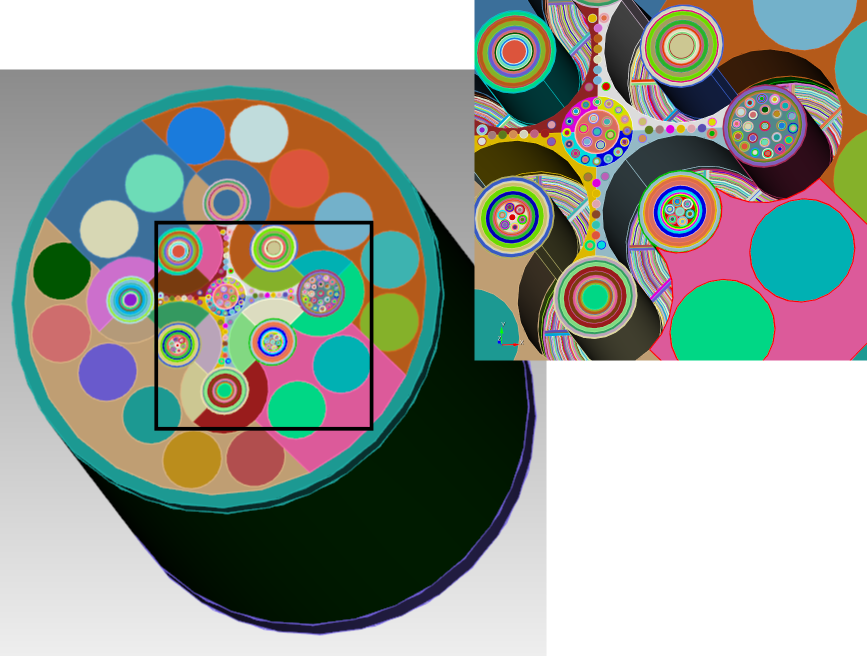
\includegraphics[height=0.4\textheight]{./images/atr_both.png} &


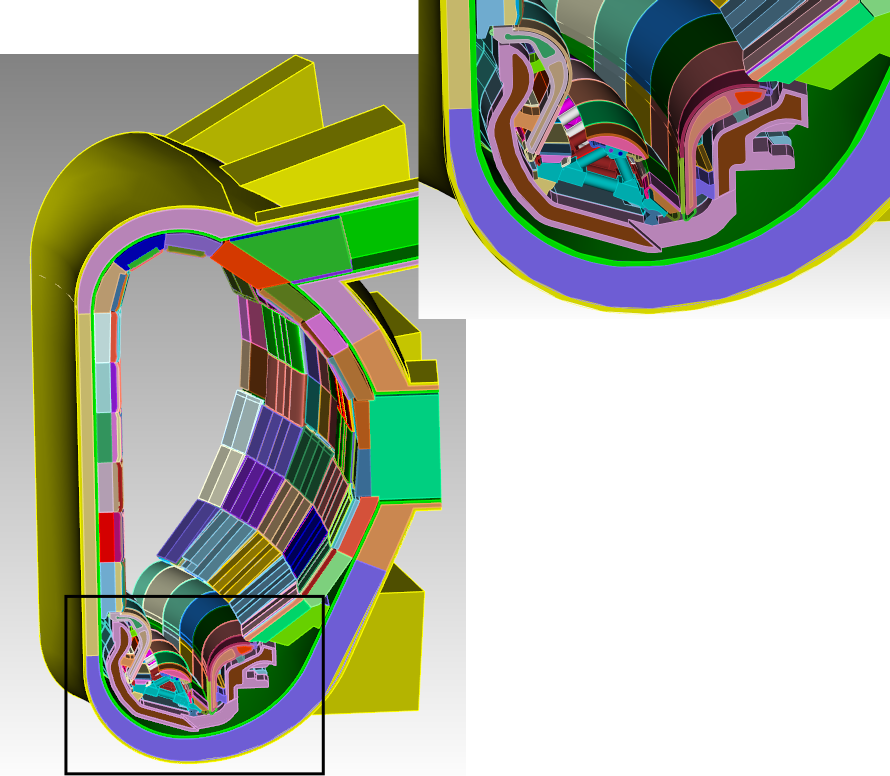
\includegraphics[height=0.4\textheight]{./images/bllite_both.png} \\

Advanced Test Reactor &

ITER \\
\end{tabular}
\end{center}

But it takes a long time... (2-10x slower than native codes)

\end{frame}

\begin{frame}

\frametitle{Ray Tracing in DAGMC}

\begin{itemize}
  \item Used for our geometric queries:
    \begin{itemize}
      \item point-inclusion tests
      \item next surface distance determination
    \end{itemize}
\end{itemize}


\end{frame}
% We use it for our geometric queries:
   % point-inclusion
   % dist to next surf
% Replaces analytic intersections in native MonteCarlo packages
% Motivation: takes too long!
% Images of typical production models?
\section{Ray Tracing Accelerations} % 2-3 slides
% BVH explanation in 1 slide
% Embree's tricks
% Extra: SAH
\section{Triangle Mesh Transfer} % 1-2 slides
% Maintaining watertightness
   % explain and refer to make_watertight
% Importance of the filter functions
   % allowed compliance with DAGMC conventions
\section{Results} % 2-3 slides
% Pure ray fire comparison (no transport)
% Single volume tests
% Multiple volume tests
\section{Drawbacks} % 2-3 slides
% Floating precision 
% Robustness needs work, triangle intersector not quite there
% Lost particles in highly complex geometries, most likely due to forced conversion
% back and forth from double to float
% Extra: slide with graphic of our specific problem
\section{Future Work} % 2 slides
% Proof of principle
% Likely to see improvements in our native system using variations of these techniques
% Point them to pyembree for a simple example of a 1-D Monte Carlo calculation in 3 regions

\begin{frame}

\end{frame}

%QUESTIONS - 1 slide

\end{document}
